\chapter{ИССЛЕДОВАНИЕ ТОЧНОСТИ ПОСТРОЕНИЯ ГЕОДЕЗИЧЕСКИХ СЕТЕЙ ПРИ УРАВНИВАНИИ СЕТЕЙ В ДИАПАЗОНАХ
	РАССТОЯНИЙ ОТ~700 ДО 1600~КМ}\label{ch:ch4}

\section{Исследование точности при построении геодезической сети в диапазоне расстояний от~700 до 1000~км}\label{sec:ch4/sect1}

На рисунке \cref{fig:pic41} приведена схема создаваемой сети при использовании РРР-алгоритма. В качестве исходных данных были получены RINEX-файлы с пунктов сети базовых станций EFT~COORS.


\begin{figure}[!h]
	\centering
	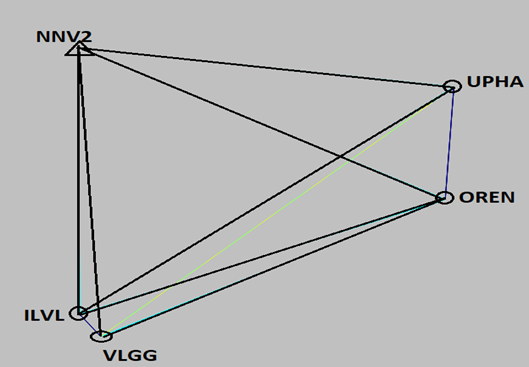
\includegraphics[width=0.99\linewidth]{images/pic41}
	\caption{Cхема сети }
	\label{fig:pic41}
\end{figure}


Геодезическая сеть состоит из пяти пунктов, равномерно расположенных в диапазоне расстояний от~$700$ до $1000$~км. Среднее расстояние между пунктами --- $850$~км.

Как и прежде, происходила обработка RINEX файлов с использованием интернет-сервиса CSRS. Для контроля получаемой точности выполнена обработка в программном обеспечении Trimble Business Centre (далее «TBC») и в статике с использованием ПО~«КРЕДО ГНСС». В последствии получены вектора и выполнено уравнивание с оценкой точности, результаты которой приведены в таблице \cref{tab:tab59}.


\begin{table} [htbp]
	\centering\small
	\begin{threeparttable}% выравнивание подписи по границам таблицы
		\captionof{table}{Оценка точности при уравнивании}\label{tab:tab59}
		\setlength{\tabcolsep}{15pt}
		\sisetup{
			table-figures-integer = 3
		}{
			\begin{tabular}{lcccccc}
				\toprule %\hline
				\textbf{~}	& \multicolumn{2}{c}{ \textbf{RTX-TBC} }	& \multicolumn{2}{c}{ \textbf{CRSR} }	& \multicolumn{2}{c}{ \textbf{статика кредо} }	\\ %\hline
				\textbf{Интервал}	& 	$\mathbf{m_{xy}}$\textbf{, м}	& $\mathbf{m_{z}}$\textbf{, м}	&
							  			$\mathbf{m_{xy}}$\textbf{, м}	& $\mathbf{m_{z}}$\textbf{, м}	& 
							  			$\mathbf{m_{xy}}$\textbf{, м}	& $\mathbf{m_{z}}$\textbf{, м}	\\ %\hline
				\midrule
				$\mathbf{1}$~ч.	& $0,023$	& $0,032$	& $0,021$	& $0,029$	& $0,095$	& $0,119$	\\ %\hline
				$\mathbf{2}$~ч.	& $0,022$	& $0,031$	& $0,019$	& $0,027$	& $0,093$	& $0,115$	\\ %\hline
				$\mathbf{3}$~ч.	& $0,021$	& $0,030$	& $0,018$	& $0,026$	& $0,089$	& $0,102$	\\ %\hline
				$\mathbf{4}$~ч.	& $0,021$	& $0,030$	& $0,018$	& $0,026$	& $0,086$	& $0,097$	\\ %\hline
				
				\bottomrule
			\end{tabular}
		}
	\end{threeparttable}
\end{table}

Как видно из таблицы \cref{tab:tab59} точность определения по РРР-алгоритму сопоставима между собой и несколько превосходит точность, получаемую в статике.



\section{Исследование точности при построении геодезической сети в диапазоне расстояний от~1000 до 1300~км}\label{sec:ch4/sect2}

На рисунке \cref{fig:pic42} приведена схема создаваемой сети при использовании РРР-алгоритма. В качестве исходных данных были получены RINEX-файлы с пунктов сети базовых станций EFT COORS.


\begin{figure}[!h]
	\centering
	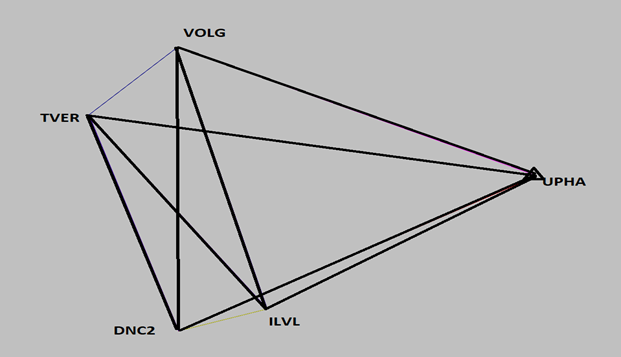
\includegraphics[width=0.99\linewidth]{images/pic42}
	\caption{Cхема сети }
	\label{fig:pic42}
\end{figure}

Геодезическая сеть состоит из пяти пунктов, равномерно расположенных в диапазоне расстояний от~$1000$ до $1300$~км. В рамках сети происходит определение восьми векторов. Для выполнения работ требуется два сеанса измерений для обеспечения их независимости.

Как и прежде, происходила обработка RINEX файлов с использованием интернет-сервиса CSRS. Для контроля получаемой точности выполнена обработка в программном обеспечении TBC и в статике с использованием ПО~«КРЕДО ГНСС». Подробнее с процессами обработки можно ознакомиться [$\ldots$]. В таблице \cref{tab:tab60} приводится оценка точности.


\begin{table} [htbp]
	\centering\small
	\begin{threeparttable}% выравнивание подписи по границам таблицы
		\captionof{table}{Оценка точности при уравнивании}\label{tab:tab60}
		\setlength{\tabcolsep}{15pt}
		\sisetup{
			table-figures-integer = 3
		}{
			\begin{tabular}{lcccccc}
				\toprule %\hline
				\textbf{~}	& \multicolumn{2}{c}{ \textbf{RTX-TBC} }	& \multicolumn{2}{c}{ \textbf{CRSR} }	& \multicolumn{2}{c}{ \textbf{статика кредо} }	\\ %\hline
				\textbf{Интервал}	& 	$\mathbf{m_{xy}}$\textbf{, м}	& $\mathbf{m_{z}}$\textbf{, м}	&
				$\mathbf{m_{xy}}$\textbf{, м}	& $\mathbf{m_{z}}$\textbf{, м}	& 
				$\mathbf{m_{xy}}$\textbf{, м}	& $\mathbf{m_{z}}$\textbf{, м}	\\ %\hline
				\midrule
				$\mathbf{1}$~ч.	& $0,040$	& $0,041$	& $0,040$	& $0,042$	& $0,252$	& $0,407$	\\ %\hline
				$\mathbf{2}$~ч.	& $0,037$	& $0,038$	& $0,039$	& $0,039$	& $0,243$	& $0,337$	\\ %\hline
				$\mathbf{3}$~ч.	& $0,036$	& $0,038$	& $0,037$	& $0,038$	& $0,196$	& $0,290$	\\ %\hline
				$\mathbf{4}$~ч.	& $0,033$	& $0,037$	& $0,037$	& $0,038$	& $0,185$	& $0,246$	\\ %\hline
				
				\bottomrule
			\end{tabular}
		}
	\end{threeparttable}
\end{table}

Как видно из таблицы \cref{tab:tab60} точность при уравнивании по РРР-алгоритму, по-прежнему, сопоставима между собой и на порядок выше, чем при классической обработке в статике.




\section{Исследование точности при построении геодезической сети в диапазоне расстояний от~1300 до 1700~км}\label{sec:ch4/sect3}

На рисунке \cref{fig:pic43} приведена схема создаваемой сети при использовании РРР-алгоритма. В качестве исходных данных были получены RINEX-файлы с пунктов сети базовых станций EFT COORS.


\begin{figure}[!h]
	\centering
	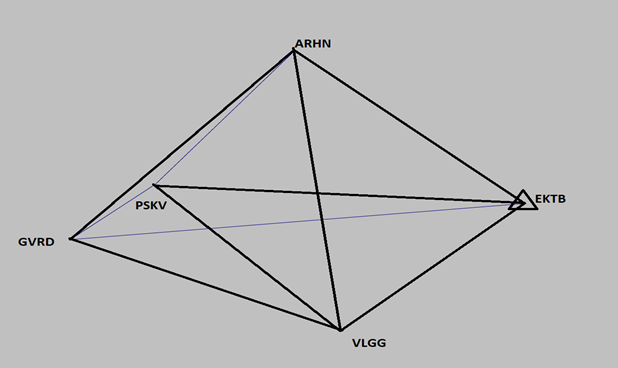
\includegraphics[width=0.99\linewidth]{images/pic43}
	\caption{Cхема сети }
	\label{fig:pic43}
\end{figure}

Геодезическая сеть состоит из пяти пунктов, равномерно расположенных в диапазоне расстояний от~$1\mathbf{4}00$ до $1900$~км. 
\footnote{Так до какого, всётаки расстояния? 1700~км, как в заголовке раздела? Или 1600~км, как в заголовке Главы? Или 1900~км, здесь? ;) }
В рамках сети происходит определение восьми векторов. Для выполнения работ требуется два сеанса измерений для обеспечения их независимости.

Как и прежде, происходила обработка RINEX файлов с использованием интернет-сервиса CSRS. Для контроля получаемой точности выполнена обработка в программном обеспечении TBC и в статике с использованием ПО~«КРЕДО ГНСС». Подробнее с процессами обработки можно ознакомиться [$\ldots$]. В таблице \cref{tab:tab61} приводится оценка точности.


\begin{table} [htbp]
	\centering\small
	\begin{threeparttable}% выравнивание подписи по границам таблицы
		\captionof{table}{Оценка точности при уравнивании}\label{tab:tab61}
		\setlength{\tabcolsep}{15pt}
		\sisetup{
			table-figures-integer = 3
		}{
			\begin{tabular}{lcccccc}
				\toprule %\hline
				\textbf{~}	& \multicolumn{2}{c}{ \textbf{RTX-TBC} }	& \multicolumn{2}{c}{ \textbf{CRSR} }	& \multicolumn{2}{c}{ \textbf{статика кредо} }	\\ %\hline
				\textbf{Интервал}	& 	$\mathbf{m_{xy}}$\textbf{, м}	& $\mathbf{m_{z}}$\textbf{, м}	&
				$\mathbf{m_{xy}}$\textbf{, м}	& $\mathbf{m_{z}}$\textbf{, м}	& 
				$\mathbf{m_{xy}}$\textbf{, м}	& $\mathbf{m_{z}}$\textbf{, м}	\\ %\hline
				\midrule
				$\mathbf{1}$~ч.	& $0,048$	& $0,051$	& $0,049$	& $0,052$	& $0,402$	& $0,290$	\\ %\hline
				$\mathbf{2}$~ч.	& $0,047$	& $0,050$	& $0,048$	& $0,049$	& $0,368$	& $0,263$	\\ %\hline
				$\mathbf{3}$~ч.	& $0,046$	& $0,049$	& $0,047$	& $0,048$	& $0,335$	& $0,242$	\\ %\hline
				$\mathbf{4}$~ч.	& $0,046$	& $0,049$	& $\mathbf{0,037} - ?$	& $0,048$	& $0,290$	& $0,215$	\\ %\hline
				
				\bottomrule
			\end{tabular}
		}
	\end{threeparttable}
\end{table}

Как видно из таблицы \cref{tab:tab61} точность при уравнивании по РРР-алгоритму, по-прежнему, сопоставима между собой и на порядок выше, чем при классической обработке в статике.

